\documentclass[a4paper,12pt]{article}

% Set of commands used by cv.tex

\usepackage[dvipsnames,usenames]{color}
\usepackage{geometry}
\usepackage{graphicx}
\usepackage{subcaption}
\usepackage{fontspec,xunicode}
\usepackage{hyperref}
\usepackage{multirow}
\usepackage{array}
\usepackage{polyglossia}
\usepackage{ragged2e}

\geometry{
    paper=a4paper,
    bindingoffset=0cm,
    top=1.5cm,
    bottom=2cm,
    left=1.0cm,
    right=2.0cm
}

\setdefaultlanguage{slovak}
\setotherlanguage{english}

% starting commands

\defaultfontfeatures{Mapping=tex-text,Scale=MatchLowercase,Ligatures={Common}}
%\setmainfont{Junicode}
\setmainfont{DejaVu Sans}
\newcommand{\largeskip}[0]{\vspace{2.5mm}\\}
\newcommand{\shortskip}[0]{\vspace{0.4mm}\\}
\setlength{\extrarowheight}{0.5mm}
% small caps
% \newcommand{\smcp}[1]{{\font\1="Junicode:+smcp" at 11pt \1{#1}}}
%\renewcommand{\textsc}[1]{\smcp{#1}}
\newcommand{\smcp}[1]{\textsc{\small\textbf{#1}}}

% \newcommand{\hsmcp}[1]{{\font\1="Junicode:+smcp" at 14pt \1{#1}}}
% \renewcommand{\textsc}[1]{\hsmcp{#1}}
\newcommand{\hsmcp}[1]{\textsc{\large#1}}

%\newcommand{\header}[3]{
%\hspace{0cm}
%\raggedright{\headline{#1}}
%\begin{tabular}{p{10cm}p{10cm}}
%{#2} & {\raggedleft{#3}} \\
%\end{tabular}
%\bigskip}
\newcommand{\header}[2]{
{\headline{#1}}\\
\shortskip
\raggedright{\large #2}
\largeskip
}

\newcommand{\blocktitle}[1]{
\parbox{\textwidth}{
	\vspace{2mm}
	\noindent
	\textcolor{MidnightBlue}{
{%\font\1="Junicode" at 16pt \1{#1}
	{\Large #1}
	\vspace*{1mm}
	\hrule}
	\vspace*{3mm}
	\noindent
} } }

%\newcommand{\headline}[1]{ {\font\1="Junicode" at 18pt \1{#1}}}
%\newcommand{\setmainfont}[0]{\font\x="Junicode" at 12pt \x}
\newcommand{\headline}[1]{\huge #1}
%%%%%%

\newenvironment{sirsiaTabulka}
{\begin{tabular}[t]{p{3.2cm}p{15cm}}}
{\end{tabular}}

\newenvironment{uzsiaTabulka}
{\begin{tabular}[t]{p{3.2cm}p{10cm}}}
{\end{tabular}}

\newenvironment{tabularblock}
{\begin{tabular}[t]{p{2.9cm}p{15cm}}}
{\end{tabular}}

%\newcommand{\zvyraznenyDvojriadok}[2]{\noindent\raggedright{\small\bfseries{\uppercase{#1}}} & #2 \tabularnewline}
\newcommand{\zvyraznenyDvojriadok}[2]{\noindent\raggedright{\small\bfseries{#1}} & #2 \tabularnewline}
\newcommand{\dvojriadok}[2]{\noindent\raggedright{#1} & {#2} \tabularnewline}
%\newcommand{\sekcia}[2]{\noindent\raggedright{\textsc{#1}} & #2 \tabularnewline}
%\newcommand{\sectionitem2}[4]{{\noindent\raggedright{\textsc{#1}}} & \raggedright{{\bf#2} {\texttt{\small #3}} \\ {#4}} \tabularnewline}
	%\newcommand{\sekcia2}[4]{{\noindent\raggedright{\textsc{#1}}} & \raggedright{{\textbf{#2} {#3}} \\ {#4}} \tabularnewline}

%%%%%%

\newcommand{\interest}[2]{
\includegraphics[height=17pt]{#1}
~\raisebox{4pt}{#2}}

%%%%%%

\newenvironment{interestsblock}[1]
{\blocktitle{#1}\begin{tabular}{p{10cm}p{10cm}}}
{\end{tabular}}

\setlength{\parindent}{0mm}
\pagestyle{empty}

% For \email{ADDRESS}, links ADDRESS to the url mailto:ADDRESS
\newcommand*\email[1]{\href{mailto:#1}{#1}}
% Same as above, but pretty-prints ADDRESS in teletype fixed-width font
\renewcommand*\email[1]{\href{mailto:#1}{\texttt{#1}}}
\newcommand{\blankline}{\quad\pagebreak[3]}
\newcommand{\halfblankline}{\quad\vspace{-0.5\baselineskip}\pagebreak[3]}


\newcommand{\datumPretekov}{1.~júna~2024 (sobota)}
\title{
	Spoznaj Les 2024 \\[1ex]
	\large \datumPretekov \\
	7.~kolo oblastného rebríčka Západnej oblasti v OB\\
	Propozície}
\author{Viktor Tomkovič}
\begin{document}
\catcode`\"=\active \def "{\begingroup„\def "{\endgroup“}}

%\maketitle

		\begin{tabular}[t]{p{6cm}p{2.5cm}p{2.5cm}p{6cm}}
	\centering \includegraphics[height=2.0cm]{logo_SZOŠ.jpg} &
	\centering 
\includegraphics[height=2.0cm]{logo_Sandberg.png} &
	\centering 
\includegraphics[height=2.0cm]{logo_Ioan.png} &
	\centering 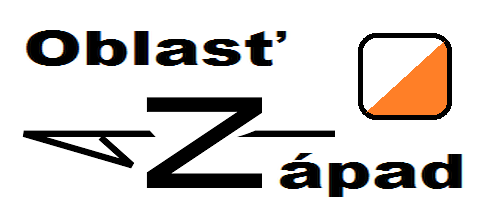
\includegraphics[height=2.0cm]{logo_ZO.png}
\end{tabular}

%\begin{figure}
%\centering
%\begin{subfigure}{0.36\textwidth}
%\centering
%\includegraphics[height=1.5cm]{logo_SZOŠ.jpg}
%\label{fig:center}
%\end{subfigure}
%\begin{subfigure}{0.27\textwidth}
%\centering
%
\includegraphics[height=2cm]{logo_Sandberg.png}
%\label{fig:left}
%\end{subfigure}
%\begin{subfigure}{0.35\textwidth}
%\centering
%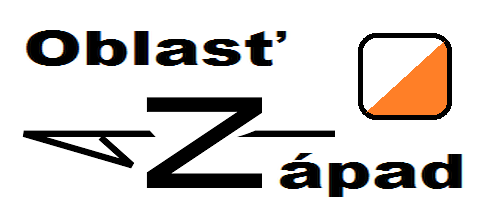
\includegraphics[height=2cm]{logo_ZO.png}
%\label{fig:right}
%\end{subfigure}
%\label{fig:combined}
%\end{figure}

\begin{center}
{
	\LARGE \textbf{Spoznaj Les 2024} \\[1ex]
\Large
%\datumPretekov  \\[0.2ex]
7.~kolo oblastného  rebríčka Západnej oblasti v OB \\
Propozície \\ 
}
\end{center}

%\medskip
\smallskip

\begin{sirsiaTabulka}
	\zvyraznenyDvojriadok{Organizátor}{Športový klub Sandberg a TJ Ioan 1209}
	\zvyraznenyDvojriadok{Dátum}{\datumPretekov }
%	\zvyraznenyDvojriadok{Miesto}{Pekná cesta nad Horárňou Krasňany}
	\zvyraznenyDvojriadok{Klasifikácia a zaradenie}{Otvorené jednorázové denné preteky jednotlivcov s určeným poradím KS na predĺžených stredných tratiach. Preteky sú 7.~kolom oblastného rebríčka pre Západnú oblasť SZOŠ.}
	\zvyraznenyDvojriadok{Umiestnenie centra}
		{Lúka Slalomka. \newline
			\href{https://sk.mapy.cz/s/hokarevoru}{https://sk.mapy.cz/s/hokarevoru} \newline
			\href{https://maps.app.goo.gl/ZHozdcu41ooa6nxHA}{https://maps.app.goo.gl/ZHozdcu41ooa6nxHA} \newline
			\href{https://osm.org/go/0LBLEbnA--?way=119767698}{https://osm.org/go/0LBLEbnA--?way=119767698}
		}
	\zvyraznenyDvojriadok{Doprava}{
		Od zástavky Potočná 750~m peši. Pri zástavke je možnosť parkovať v obmedzenom množstve. Odporúčame nespoliehať sa na túto možnosť a zaparkovať nižšie v Rači.
		Autobus č.~52 premáva zo zástavky Detvianská s odchodom o 8:07, potom každých 30~minút.
	}
	\zvyraznenyDvojriadok{Štart}{
		\begin{uzsiaTabulka}
			\dvojriadok{10:00 -- 11:00}{Rebríčkové kategórie -- voľný intervalový štart}
			\dvojriadok{10:00 -- 12:00}{Verejné kategórie -- voľný intervalový štart}
		\end{uzsiaTabulka}
	}
	\zvyraznenyDvojriadok{Kategórie}{
		\begin{uzsiaTabulka}
				\dvojriadok{Rebríčkové}{M 10, M 12, M 14, M 16, M 18, M 19, M 40, M 55, M 70, Open,\newline
			W 10, W 12, W 14, W 16, W 18, W 19, W 40, W 55, W 70}
				\dvojriadok{Verejné}{MWR -- deti s doprovodom, N -- nováčikovia, Verejnosť -- široká verejnosť/zvedaví okoloidúci, Obrázková detská trať} % napis Edite
				% kto bude robit layout map - informacie pre verejnost na verejnej mape
		\end{uzsiaTabulka}
	}
\end{sirsiaTabulka}
\begin{sirsiaTabulka}
	\zvyraznenyDvojriadok{Štartovné}{
		\begin{obratenaTabulka}
			\dvojriadok{MW~18, MW~19, MW~40, MW~55, MW~70, Open}{7€}
			\dvojriadok{MW~10, MW~12, MW~14, MW~16, N, MWR, Verejnosť}{5€}
		\end{obratenaTabulka}
		\begin{uzsiaTabulka}
				\dvojriadok{Kluby:}{Iba prevodom na účet SK90~8330~0000~0020~0178~4563}
				\dvojriadok{Jednotlivci:}{Cez IS SZOŠ alebo v hotovosti počas prezentácie.}
		\end{uzsiaTabulka}
	}
	\zvyraznenyDvojriadok{Prihlášky}{Pomocou prihlasovacieho systému \href{https://is.orienteering.sk/competitions/1857}{IS SZOŠ} najneskôr do 27.~5.~2024. \newline
	\href{https://is.orienteering.sk/competitions/1857}{https://is.orienteering.sk/competitions/1857} \newline
Neregistrovaní pretekári sa prihlasujú cez informačný systém SZOŠ (treba si v
	ňom vytvoriť konto), alebo mailom na \email{sandberg.orienteering@gmail.com} v
rovnakých termínoch. Verejnosť sa môže prihlásiť priamo v centre pretekov do 12:00.

Po termíne s 50\% prirážkou okrem verejných kategórií (N, MWR, Verejnosť).

Odhlášky po zadaní máp do tlače sa neakceptujú.

Prihlášky mailom sú platné až po písomnom potvrdení.
	}% skopiruj zo Snezienok a Machrov
\end{sirsiaTabulka}
\begin{sirsiaTabulka}
	\zvyraznenyDvojriadok{Prezentácia}{V centre pretekov v deň konania pretekov v čase od 8:30 do 9:30, verejnosť a detská obrázková trať do 12:00. \newline
		Kluby a jednotlivci s riadne uhradeným štartovným a bez zmien sa nemusia prezentácie zúčastniť.
	} % Do pokynov pridat, ze ti, co su vybaveni, sa nemusia ist prezentovat
%	\zvyraznenyDvojriadok{Poplatky}{???vklad, ostatné poplatky, spôsob platenia, pravidlá odhlášok z pretekov???}
%	\zvyraznenyDvojriadok{Ubytovacie možnosti}{Organizátor pretekov neposkytuje.}
\end{sirsiaTabulka}
\begin{sirsiaTabulka}
	\zvyraznenyDvojriadok{Smerné časy}{Dlhšie ako stredná trať (čl.~12.12.~Pravidiel~OB), kratšie ako dlhá trať (čl.~12.11.~Pravidiel~OB).}
	\zvyraznenyDvojriadok{Opis terénu}{Bratislavské mestské lesy. Listnatý les s veľkým množstvom vývratov a kôpok. Oblasť pretekov 
		obsahuje veľké zarastajúce rúbaniská. Preteky budú na úplne novej mape. Mierne zvlnený terén, dobre priebežný les.}
	% listnaty les, nova mapa, velke zarastajuce rubaniska, vela vyvratov a kopok, spolocna mapa zapadnej oblasti
%	\zvyraznenyDvojriadok{Zakázané priestory}{??? mapa?}%Sprav mapu, vymedzenie ziadostou
\end{sirsiaTabulka}
\begin{sirsiaTabulka}
	\zvyraznenyDvojriadok{Mapa}{Spoločná mapa Západnej Oblasti, mierka 1:10~000, e = 5m. Stav:~november~2023 \newline 
	\begin{tabular}[t]{p{4cm}p{4cm}p{4cm}}
		\centering 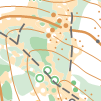
\includegraphics[height=2.0cm]{ukážka_mapy_1.png} &
		\centering 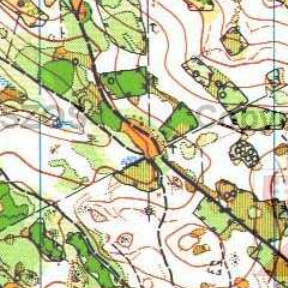
\includegraphics[height=2.0cm]{ukážka_mapy_2.png} &
		\centering 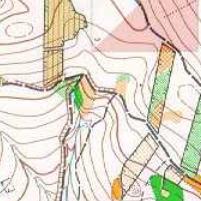
\includegraphics[height=2.0cm]{ukážka_mapy_3.png}
	\end{tabular}
	}% jesen/november 2023
	\zvyraznenyDvojriadok{Staršie mapy}{
		Bučina~(1972), \href{https://www.orienteering.sk/maps-new/jpg-gif/153.jpg}{https://www.orienteering.sk/maps-new/jpg-gif/153.jpg} \newline
		Kotliarka~(1987), \href{https://www.orienteering.sk/maps-new/jpg-gif/135.jpg}{https://www.orienteering.sk/maps-new/jpg-gif/135.jpg}% \newline
		%Snežienka~(1996), \href{https://www.orienteering.sk/maps-new/jpg-gif/270.jpg}{https://www.orienteering.sk/maps-new/jpg-gif/270.jpg}
	}%https://www.orienteering.sk/maps-new/mapy/mapa/mapa.php?j=sl&id=153
	\zvyraznenyDvojriadok{Raziaci systém}{SportIdent Air{\small\texttt +}, požičanie: čip 2€ (strata {\small\texttt +}35€), SIAC 5€ (strata {\small\texttt +}80€).}
	\zvyraznenyDvojriadok{Bližšie informácie}{e-mail: \email{sandberg.orienteering@gmail.com} \newline telefón: Viktor Tomkovič, {{\small\texttt +}421~902~229~430}}
\end{sirsiaTabulka}
	% KONIEC POVINNÝCH, ZAČIATOK OBVYKLÝCH INFORMÁCIÍ
\begin{sirsiaTabulka}
%	\zvyraznenyDvojriadok{Uzávierka cieľa}{12:30???}
%	\zvyraznenyDvojriadok{Vyhlásenie výsledkov}{13:00???}
%	\zvyraznenyDvojriadok{Opisy KS}{Dostupnosť}
%	\zvyraznenyDvojriadok{Občerstvenie}{Sandberg}
%	\zvyraznenyDvojriadok{WC}{Sandberg}
%	\zvyraznenyDvojriadok{Prvá pomoc}{Sandberg}
%	\zvyraznenyDvojriadok{Rozcvičovanie}{Sandberg}
%	\zvyraznenyDvojriadok{Parkovanie}{Sandberg}
%	\zvyraznenyDvojriadok{Vzdialenosti}{Sandberg}
	\zvyraznenyDvojriadok{Obrázková trať}{Detská obrázková trať bude k dispozícii medzi 10:00 a 12:00 v priestore zhromaždiska, bez nutnosti registrácie.}
	\zvyraznenyDvojriadok{Verejnosť}{Verejná trať bude k dispozícii medzi 10:00 a 12:00 v okolí zhromaždiska, bez nutnosti registrácie. Štartovné je 5€.}
	\zvyraznenyDvojriadok{Pravidlá}{Preteká sa podľa Pravidiel OB pre rok 2024.}
%	\zvyraznenyDvojriadok{Poznámka}{Dodržiavajte zákazy plynúce z mapových symbolov, obzvlášť
%dbajte na symbol 528.1 - Oblasť so zákazom vstupu.
%V priestore pretekov budú vytvorené umelé prekážky, v teréne
%označené páskou a na mape symbolom 707 - Neprekročiteľná
%hranica a 709 - Neprístupná oblasť. Zákazy budú kontrolované
%rozhodcami.
%Mapy sa v cieli neodovzdávajú, žiadame o dodržiavanie pravidiel
%fair play. Pretekári v cieli neukazujte svoju mapu pretekárom pred
%štartom!
%Žiadame pretekárov, ktorí štartujú aj ako sprievod v kategórii
%MWR, aby najskôr absolvovali svoju trať a až potom MWR.}
	\zvyraznenyDvojriadok{Organizačný tím}{
		\begin{uzsiaTabulka}
			\dvojriadok{Riaditeľ pretekov:}{Viktor Tomkovič}
			\dvojriadok{Hlavný rozhodca:}{Barbora Vorlíčková, R2}
			\dvojriadok{Staviteľ tratí:}{Peter Vorlíček, R3}
			\dvojriadok{Prezentácia:}{Marta Jonášová}
		\end{uzsiaTabulka}
	}
	\zvyraznenyDvojriadok{Upozornenie}{
Všetci štartujúci sa zúčastňujú pretekov dobrovoľne a na vlastnú
zodpovednosť, bez nároku na odškodné pri zranení alebo úraze
spôsobenom počas alebo následkom týchto pretekov.

Prihlásením sa na tieto preteky každý účastník súhlasí so
zverejnením svojich osobných údajov (meno, kategória, klubová
príslušnosť) v prihláške, štartovej listine, výsledkoch, na
internetovej stránke pretekov a v informačnom systéme SZOŠ.

Počas pretekov budú vyhotovované fotografie, za účelom
informovania verejnosti o pretekoch a tiež k osobnej potrebe
pretekárov ako spomienka na preteky, alebo propagácie
orientačného behu. V prípade, že nesúhlasíte s fotografovaním,
oznámte bezodkladne túto skutočnosť fotografovi.

Predajné a marketingové aktivity na pretekoch jedine so súhlasom riaditeľa pretekov.}
\end{sirsiaTabulka}
%https://www.orienteering.sk/page/zapadna-oblast-rebricky#Oblast
%\smallskip
\begin{center}
\begin{tabular}{ >{\centering}m{0.4 \textwidth } >{\centering}m{0.4 \textwidth } }
Barbora Vorlíčková & Viktor Tomkovič \tabularnewline
hlavná rozhodkyňa & riaditeľ pretekov
\end{tabular}
\end{center}

\begin{figure}[h!]
\centering
\begin{subfigure}{0.30\textwidth}
\centering

\includegraphics[height=1.9cm]{logo_lesyBA.png}
\end{subfigure}
\begin{subfigure}{0.30\textwidth}
\centering

\includegraphics[height=2.1cm]{logo_BSK.pdf}
\end{subfigure}
\begin{subfigure}{0.30\textwidth}
\centering

\includegraphics[height=1.9cm]{logo_BA.pdf}
\end{subfigure}
\end{figure}

\end{document}
% nase logo, logo zapadnej oblasti, tj ioan, mestske lesy, logo bsk, mesto bratislava

